\section{Design Methodology}
Throughout the project, an emphasis was placed on an iterative, test-driven design process. This testing involved both the use of smaller, well understood test cases and incremental unit tests in the context of the full system. 
The applicability of these smaller test cases stemmed from the use of the \textit{modular programming} paradigm, which will allow the same code to be used across a variety of different mechanical systems. 
A brief outline of the software tools used with this methodology will be followed by discussion of the core principals and importance of these concepts before formalizing the overarching process.
\subsection{Software Tools}
\subsubsection{Mathematica}
Due to the complex nature of the model and the large number of degrees of freedom needed to accurately model the behavior of the RipStik, a powerful symbolic computation tool is required to derive and manipulate the expressions. 
Mathematica was ultimately selected over other options such as Maple and the Matlab Symbolic toolbox due to the combination of robust symbolic and numeric computation features with easy to use visualization features for graphically displaying the various systems developed over the course of the project.
It also provided equivalent or better performance with thorough documentation and examples compared to competitors.
\subsubsection{Three.JS}
While all of the more simple visualizations were constructed directly in Mathematica, an external tool was constructed to animate the full RipStik system in a more attractive and visually intuitive manner. 
The application is javascript based and operated via the web browser, allowing the user to upload a .csv (comma separated value) file of numeric output from the RipStik simulation and returning an animation of the results on a 3 dimensional RipStik model. 
This allows easy validation of the results by inspection, particularly for complex motions where graphs of the angles and positions may not make the full system behavior immediately obvious.
The process used to generate these animations in the application is shown in Figure \ref{fig:ThreeJsFlow}.

%%Define the two block types and arrow type for our flow diagram
\tikzstyle{startstop} = [rectangle, rounded corners, minimum width=3cm, minimum height=1cm,text centered, draw=black, fill=white]
\tikzstyle{process} = [rectangle, minimum width=3cm, minimum height=1cm, text centered, draw=black, fill=white]
\tikzstyle{arrow} = [thick,->,>=stealth]
\begin{center}
	\begin{figure}[!htb]
		\begin{center}
			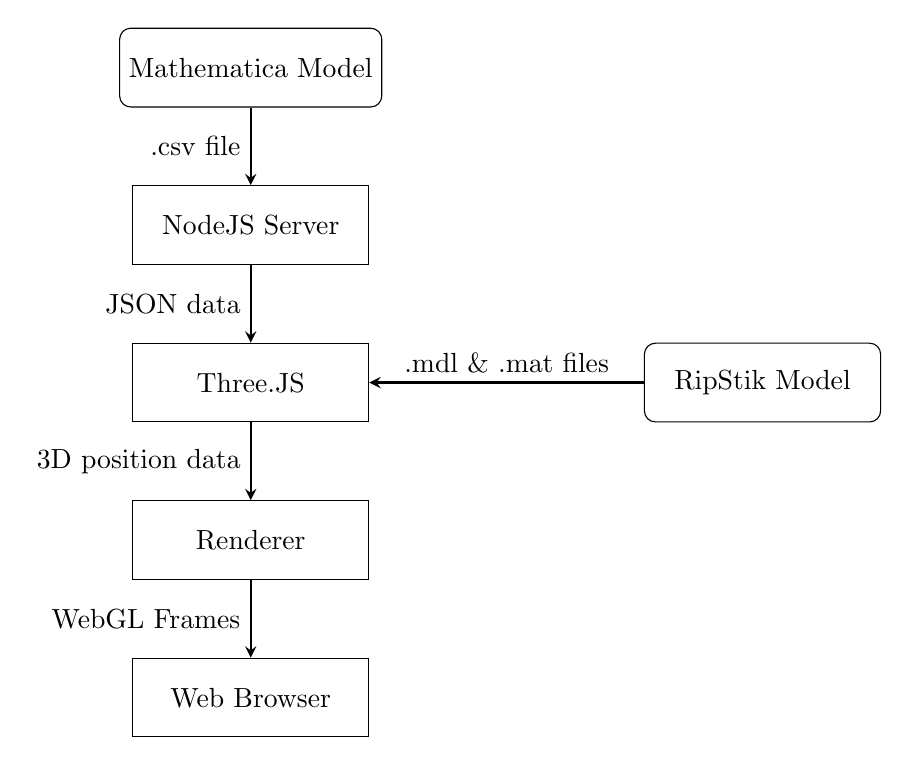
\begin{tikzpicture}[node distance=2cm]
				\node (WA) [startstop] {Mathematica Model};
				\node (Srvr) [process, below of=WA] {NodeJS Server};
				\node (Three) [process, below of=Srvr] {Three.JS};
				\node (Mdl) [startstop, right of=Three, xshift=4.5cm] {RipStik Model};
				\node (Rndr) [process, below of=Three] {Renderer};
				\node (Brwsr) [process, below of=Rndr] {Web Browser};

				\draw [arrow] (WA) -- node[anchor=east] {.csv file} (Srvr);
				\draw [arrow] (Srvr) -- node[anchor=east] {JSON data} (Three);
				\draw [arrow] (Mdl) -- node[anchor=south] {.mdl \& .mat files} (Three);
				\draw [arrow] (Three) -- node[anchor=east] {3D position data} (Rndr);
				\draw [arrow] (Rndr) -- node[anchor=east] {WebGL Frames} (Brwsr);
			\end{tikzpicture}
		\end{center}
	\caption{RipStik animation tool data flow summary}\label{fig:ThreeJsFlow}
	\end{figure}
\end{center}
The core of the application is ThreeJS, a javascript WebGL library that allows the 3D model to be loaded from a .mdl file (the set of 3D dimensional points that forms the shape) and .mat file (the colors/materials to be overlaid on the shape) then animated using rotations and translations in a standard Cartesian coordinate system.
\subsection{Modular Program Design}
The core principle of modular program design is to decompose the larger system design problem into small, independent modules\cite{Modular}.
An effective decomposition is done in such that the modules are have well defined inputs and outputs and can be tested independently, improving the flexibility of the application\cite{Modular}.
In designing the RipStik model, these modules are user created Mathematica functions, separated to each contain a complete, testable portion of the larger model.

Two alternate approaches were also considered but deemed unsuitable. Object Oriented design involves grouping related functionality and data, like parameters or variables, into larger "objects"\cite{ObjectOriented}.
This would provide similar compartmentalization \cite{ObjectOriented} but does not conform to the broader functional design of Mathematica \cite{MathematicaFunctional} and is less intuitive and legible for new users attempting to adopt code from the system. 

Alternately, a purely procedural approach would simply focus on laying out the set of commands sequentially in a single structure. 
This design would be more intuitive to new users and would likely improve initial development speed due to the lack of unit testing and reduced need for flexibility of the commands in sequence versus those implemented in independent modules.
Despite these benefits, this design was not selected since it would reduce the flexibility and testability of the system due to the purpose built nature of commands. 
This would make smaller test cases much more difficult to implement since each would be a completely independent code base with no shared functions outside of those central to Mathematica.
\subsection{Test Cases}
In order to validate each module during development, small test systems were developed. Each test system had to:
\begin{itemize}
\item Succinctly demonstrate the complete functionality of the module 
\item Be small and straightforward to minimize the time expended on setting up systems outside of the core RipStik model
\item Provide results that could be easily verified through simple visualizations and (where possible) published results
\end{itemize}
These test cases will be presented throughout the development of the model alongside the discussion of implementing each mathematical tool.
\subsection{Unit Testing}
In addition to the simple mechanical systems used to test each model, a test or set of tests was developed for the RipStik system to further validate that the given portion of the model was functioning as expected. These were designed to be as simple and easy to implement as possible while still testing the module as thoroughly as possible.
\subsection{Overall Process}
Together, modular program design, test cases and unit testing make up the core design process for each module as outlined in Figure \ref{fig:ProcessFlow}. These modules were then used to iteratively construct the overall RipStik model, adding functionality and testing incrementally for each mathematical tool applied.
\begin{center}
	\begin{figure}[!htb]
		\begin{center}
			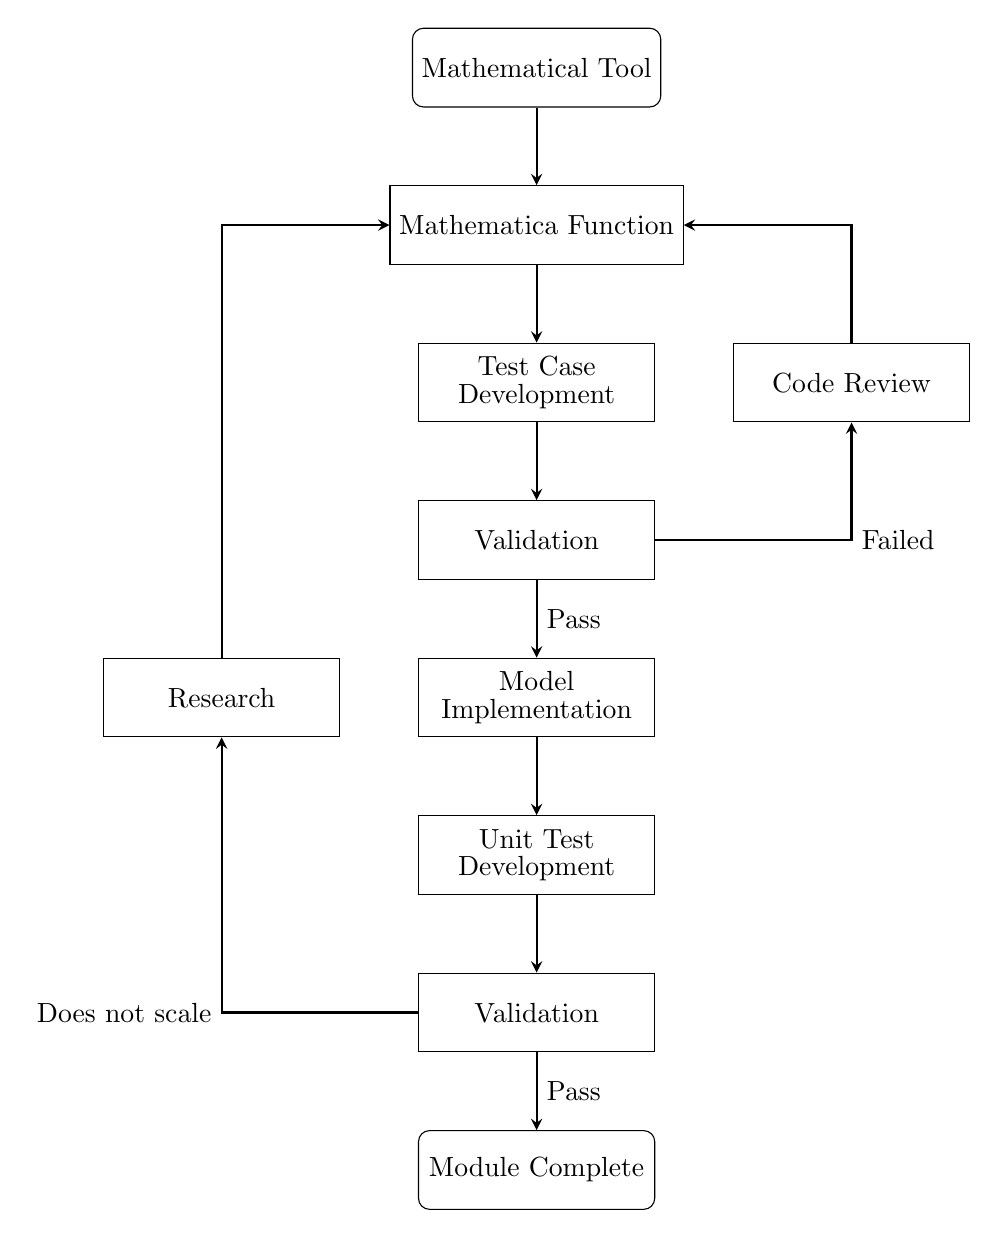
\begin{tikzpicture}[node distance=2cm]
				\node (math) [startstop] {Mathematical Tool};
				\node (code) [process, below of=math] {Mathematica Function};
				\node (testcase) [process, below of=code] {\shortstack{Test Case \\ Development}};
				\node (tcvalid) [process, below of=testcase] {Validation};
				\node (model) [process, below of=tcvalid] {\shortstack{Model \\ Implementation}};
				\node (unittest) [process, below of=model] {\shortstack{Unit Test \\ Development}};
				\node (utvalid) [process, below of=unittest] {Validation};
				\node (done) [startstop, below of=utvalid] {Module Complete};
				\node (research) [process, left of=model, node distance=4cm] {Research};
				\node (review) [process, right of=testcase, node distance=4cm] {Code Review};
				\draw [arrow] (math) -- (code);
				\draw [arrow] (code) -- (testcase);
				\draw [arrow] (testcase) -- (tcvalid);
				\draw [arrow] (tcvalid) -- node [anchor=west] {Pass}(model);
				\draw [arrow] (model) -- (unittest);
				\draw [arrow] (unittest) -- (utvalid);
				\draw [arrow] (utvalid) -- node [anchor=west] {Pass}(done);
				\draw [arrow] (utvalid) -| node [anchor=east] {Does not scale}(research);
				\draw [arrow] (research) |- (code);
				\draw [arrow] (tcvalid) -| node [anchor=west] {Failed}(review);
				\draw [arrow] (review) |- (code);
			\end{tikzpicture}
		\end{center}
	\caption{Design Process Summary Diagram}\label{fig:ProcessFlow}
	\end{figure}
\end{center}
